\documentclass[aspectratio=169]{beamer}
\usetheme[faculty=fsps]{fibeamer}
\usepackage[utf8]{inputenc}
\usepackage{ctex}
\usepackage[
  main=english, %% By using `czech` or `slovak` as the main locale
                %% instead of `english`, you can typeset the
                %% presentation in either Czech or Slovak,
                %% respectively.
  czech, slovak %% The additional keys allow foreign texts to be
]{babel}
\title{\Huge{{无线移动技术}}} %% that will be typeset on the
\subtitle{课程报告展示} %% title page.
\author{赵晨阳\ 杜⼦煜\ 章管淮\ 苗恒硕\ 钏茗喜 \\ \zhtoday}
%% These additional packages are used within the document:
\usepackage{ragged2e}  % `\justifying` text
\usepackage{booktabs}  % Tables
\usepackage{tabularx}
\usepackage{tikz}      % Diagrams
\usetikzlibrary{calc, shapes, backgrounds}
\usepackage{amsmath, amssymb}
\usepackage{url}       % `\url`s
\usepackage{listings}  % Code listings
\frenchspacing
\begin{document}
  \shorthandoff{-}
  \frame[c]{\maketitle}

  \AtBeginSection[]{% Print an outline at the beginning of sections
    \begin{frame}<beamer>
      \frametitle{目录 \thesection}
      \tableofcontents[currentsection]
    \end{frame}}

    \section{整体情况}
    \begin{frame}{整体情况}
      我们小组负责⽂图三楼的无线信号勘察工作。我们在勘察基础上,选择了上⽹体验优秀与糟糕的四处位置的⽆线⽹络状况进⾏监测与分析,并对比测试结果。现在将我们具体的实验成果进行展示。\\\bigskip
      我们组的实际测量与对应报告由赵晨阳、章管淮、苗恒硕与钏茗喜完成,而 Analyser 分析与报告由杜⼦煜同学完成。此外,赵晨阳担任小组组长,负责联络统筹全组的工作,并且两次调度实验设备。
    \end{frame}


    \section{楼层网络勘察}
    \begin{frame}{整体勘探情况}
      \begin{columns}[onlytextwidth]
        \column{.6\textwidth}
        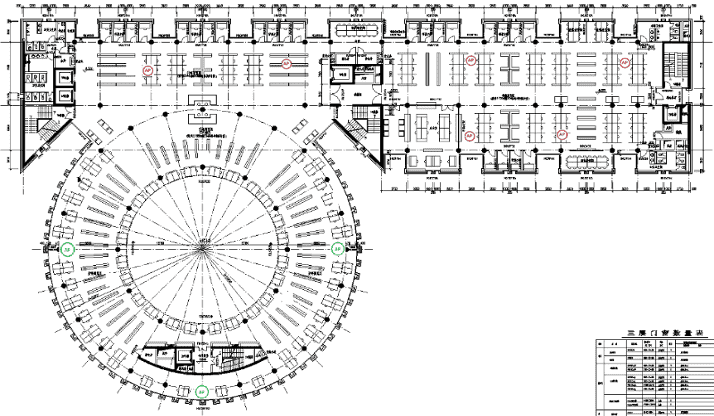
\includegraphics[width=0.8\textwidth]{resources/楼层地图.png}
        \column{.4\textwidth}
          \begin{itemize}
            \item 本小组勘察的范围是人文社科图书馆3层,总体长118m,宽64m,由矩形部分和圆环部分组成。
            \item 两部分均有图书架和座位,矩形部分另有研讨间和厕所;除此之外,测量范围还包括了楼梯间。
          \end{itemize}
      \end{columns}
    \end{frame}

    \begin{frame}{整体信号覆盖}
      \begin{columns}[onlytextwidth]
        \column{.6\textwidth}
        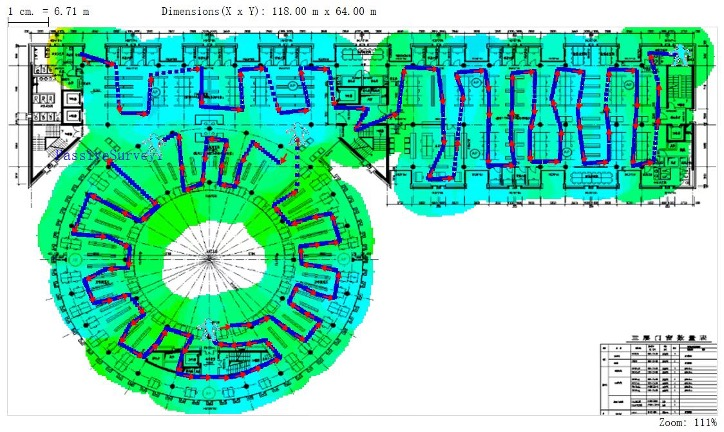
\includegraphics[width=0.8\textwidth]{resources/整体信号覆盖.png}
        \column{.4\textwidth}
          \begin{itemize}
            \item 测量路线及整体信号测量结果如图所示。
            \item 文图 3 层整体信号覆盖情况较好,只在部分区域存在信号覆盖差的情况。
          \end{itemize}
      \end{columns}
    \end{frame}

    \begin{frame}{具体信号覆盖}
        \includegraphics[width=0.9\textwidth]{resources/具体信号覆盖.png}
    \end{frame}

    \begin{frame}{AP 位置预测}
      根据整体信号覆盖情况和单 SSID 的信号分布,推理得出 AP 位置的估计如图中红色标记处:
      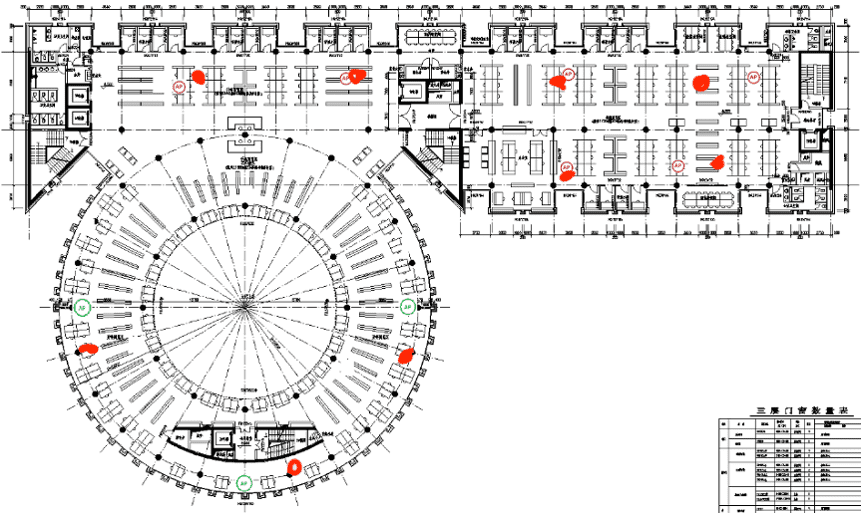
\includegraphics[width=0.7\textwidth]{resources/AP 位置预测.png}
  \end{frame}

  \begin{frame}{干扰强度分布}
    按测量路线获得文图 3 层的无线信号干扰强度分布如图:
    \includegraphics[width=0.9\textwidth]{resources/干扰强度分布.png}
  \end{frame}

    \section{定点分析}
    \begin{frame}{监测点选择}
      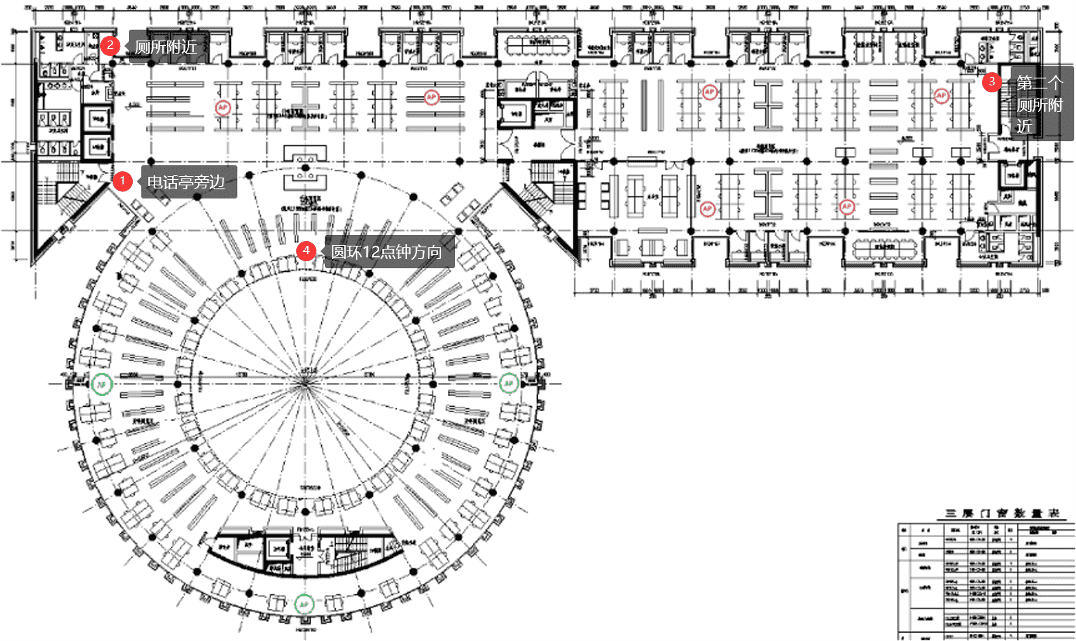
\includegraphics[width=0.8\textwidth]{resources/监测点选择.png}
    \end{frame}

    \begin{frame}{时延测试}
      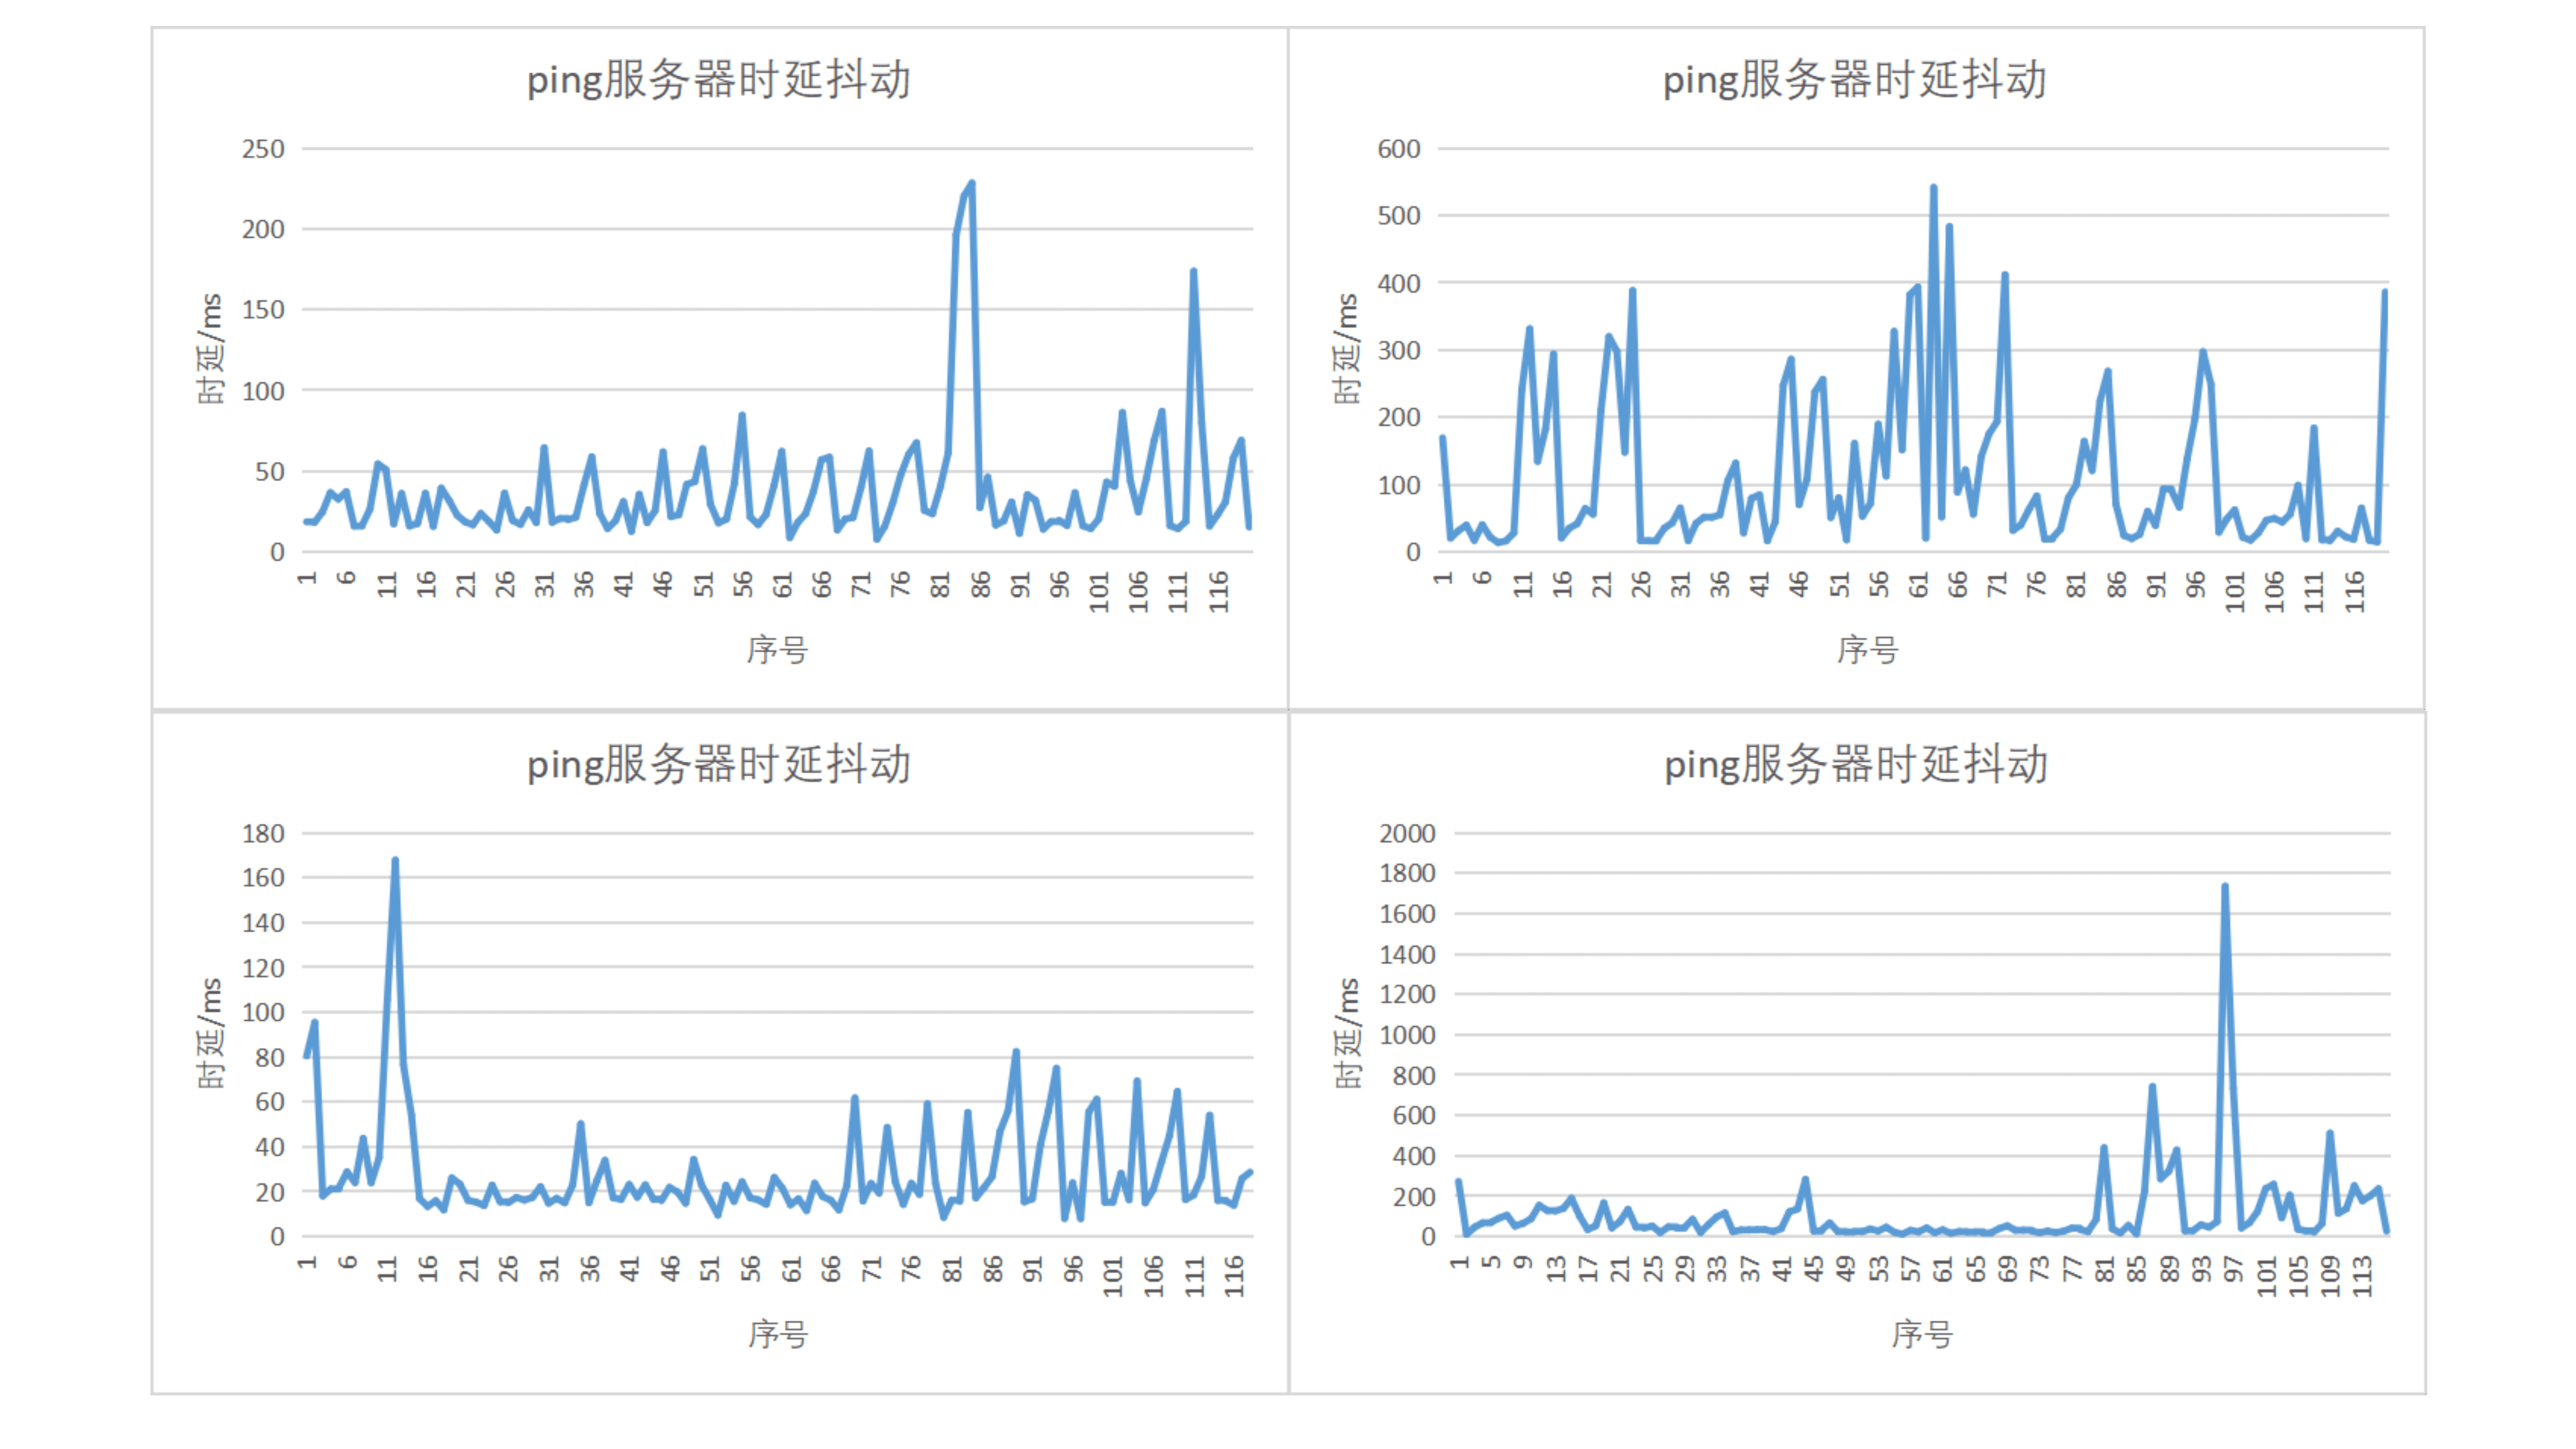
\includegraphics[width=0.9\textwidth]{resources/时延测试.png}
    \end{frame}

    \begin{frame}{吞吐量测试}
      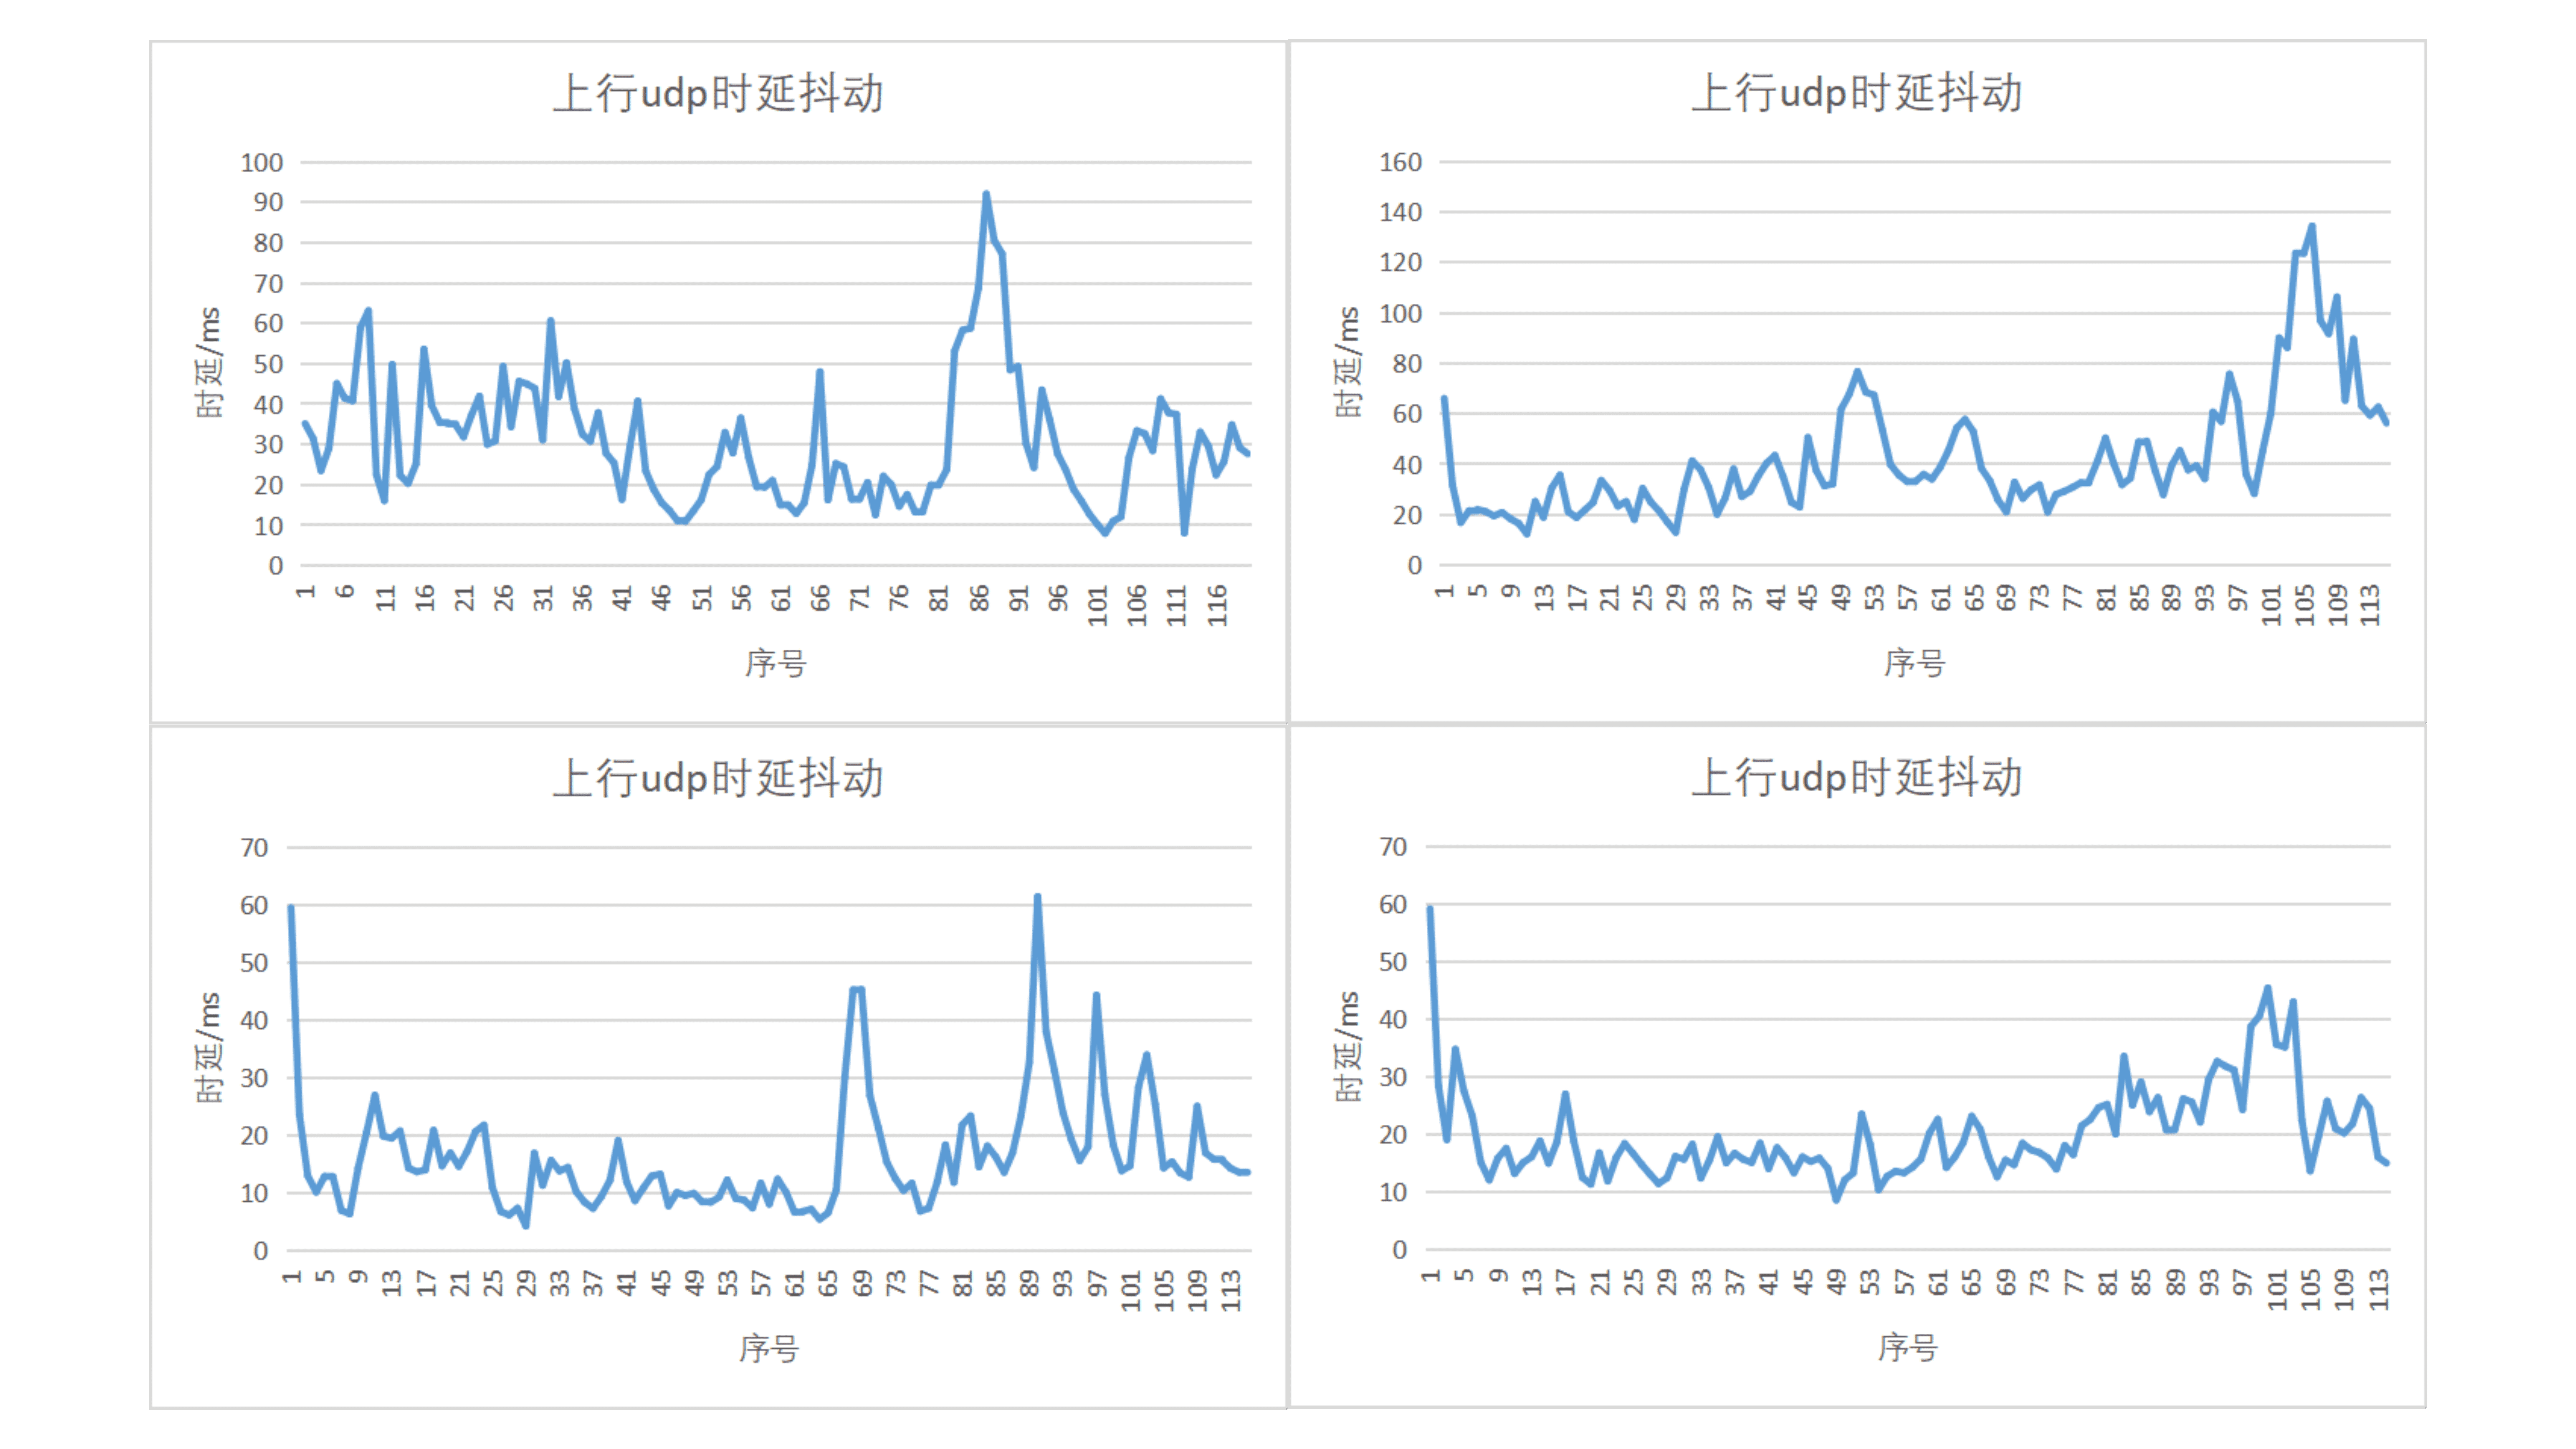
\includegraphics[width=0.9\textwidth]{resources/吞吐量测试.png}
    \end{frame}

    \section{Analyzer 分析}
    \begin{frame}{Analyzer 分析}
      \includegraphics[width=0.9\textwidth]{resources/Analyser 分析.png}
    \end{frame}

    \begin{frame}{东北角厕所}
      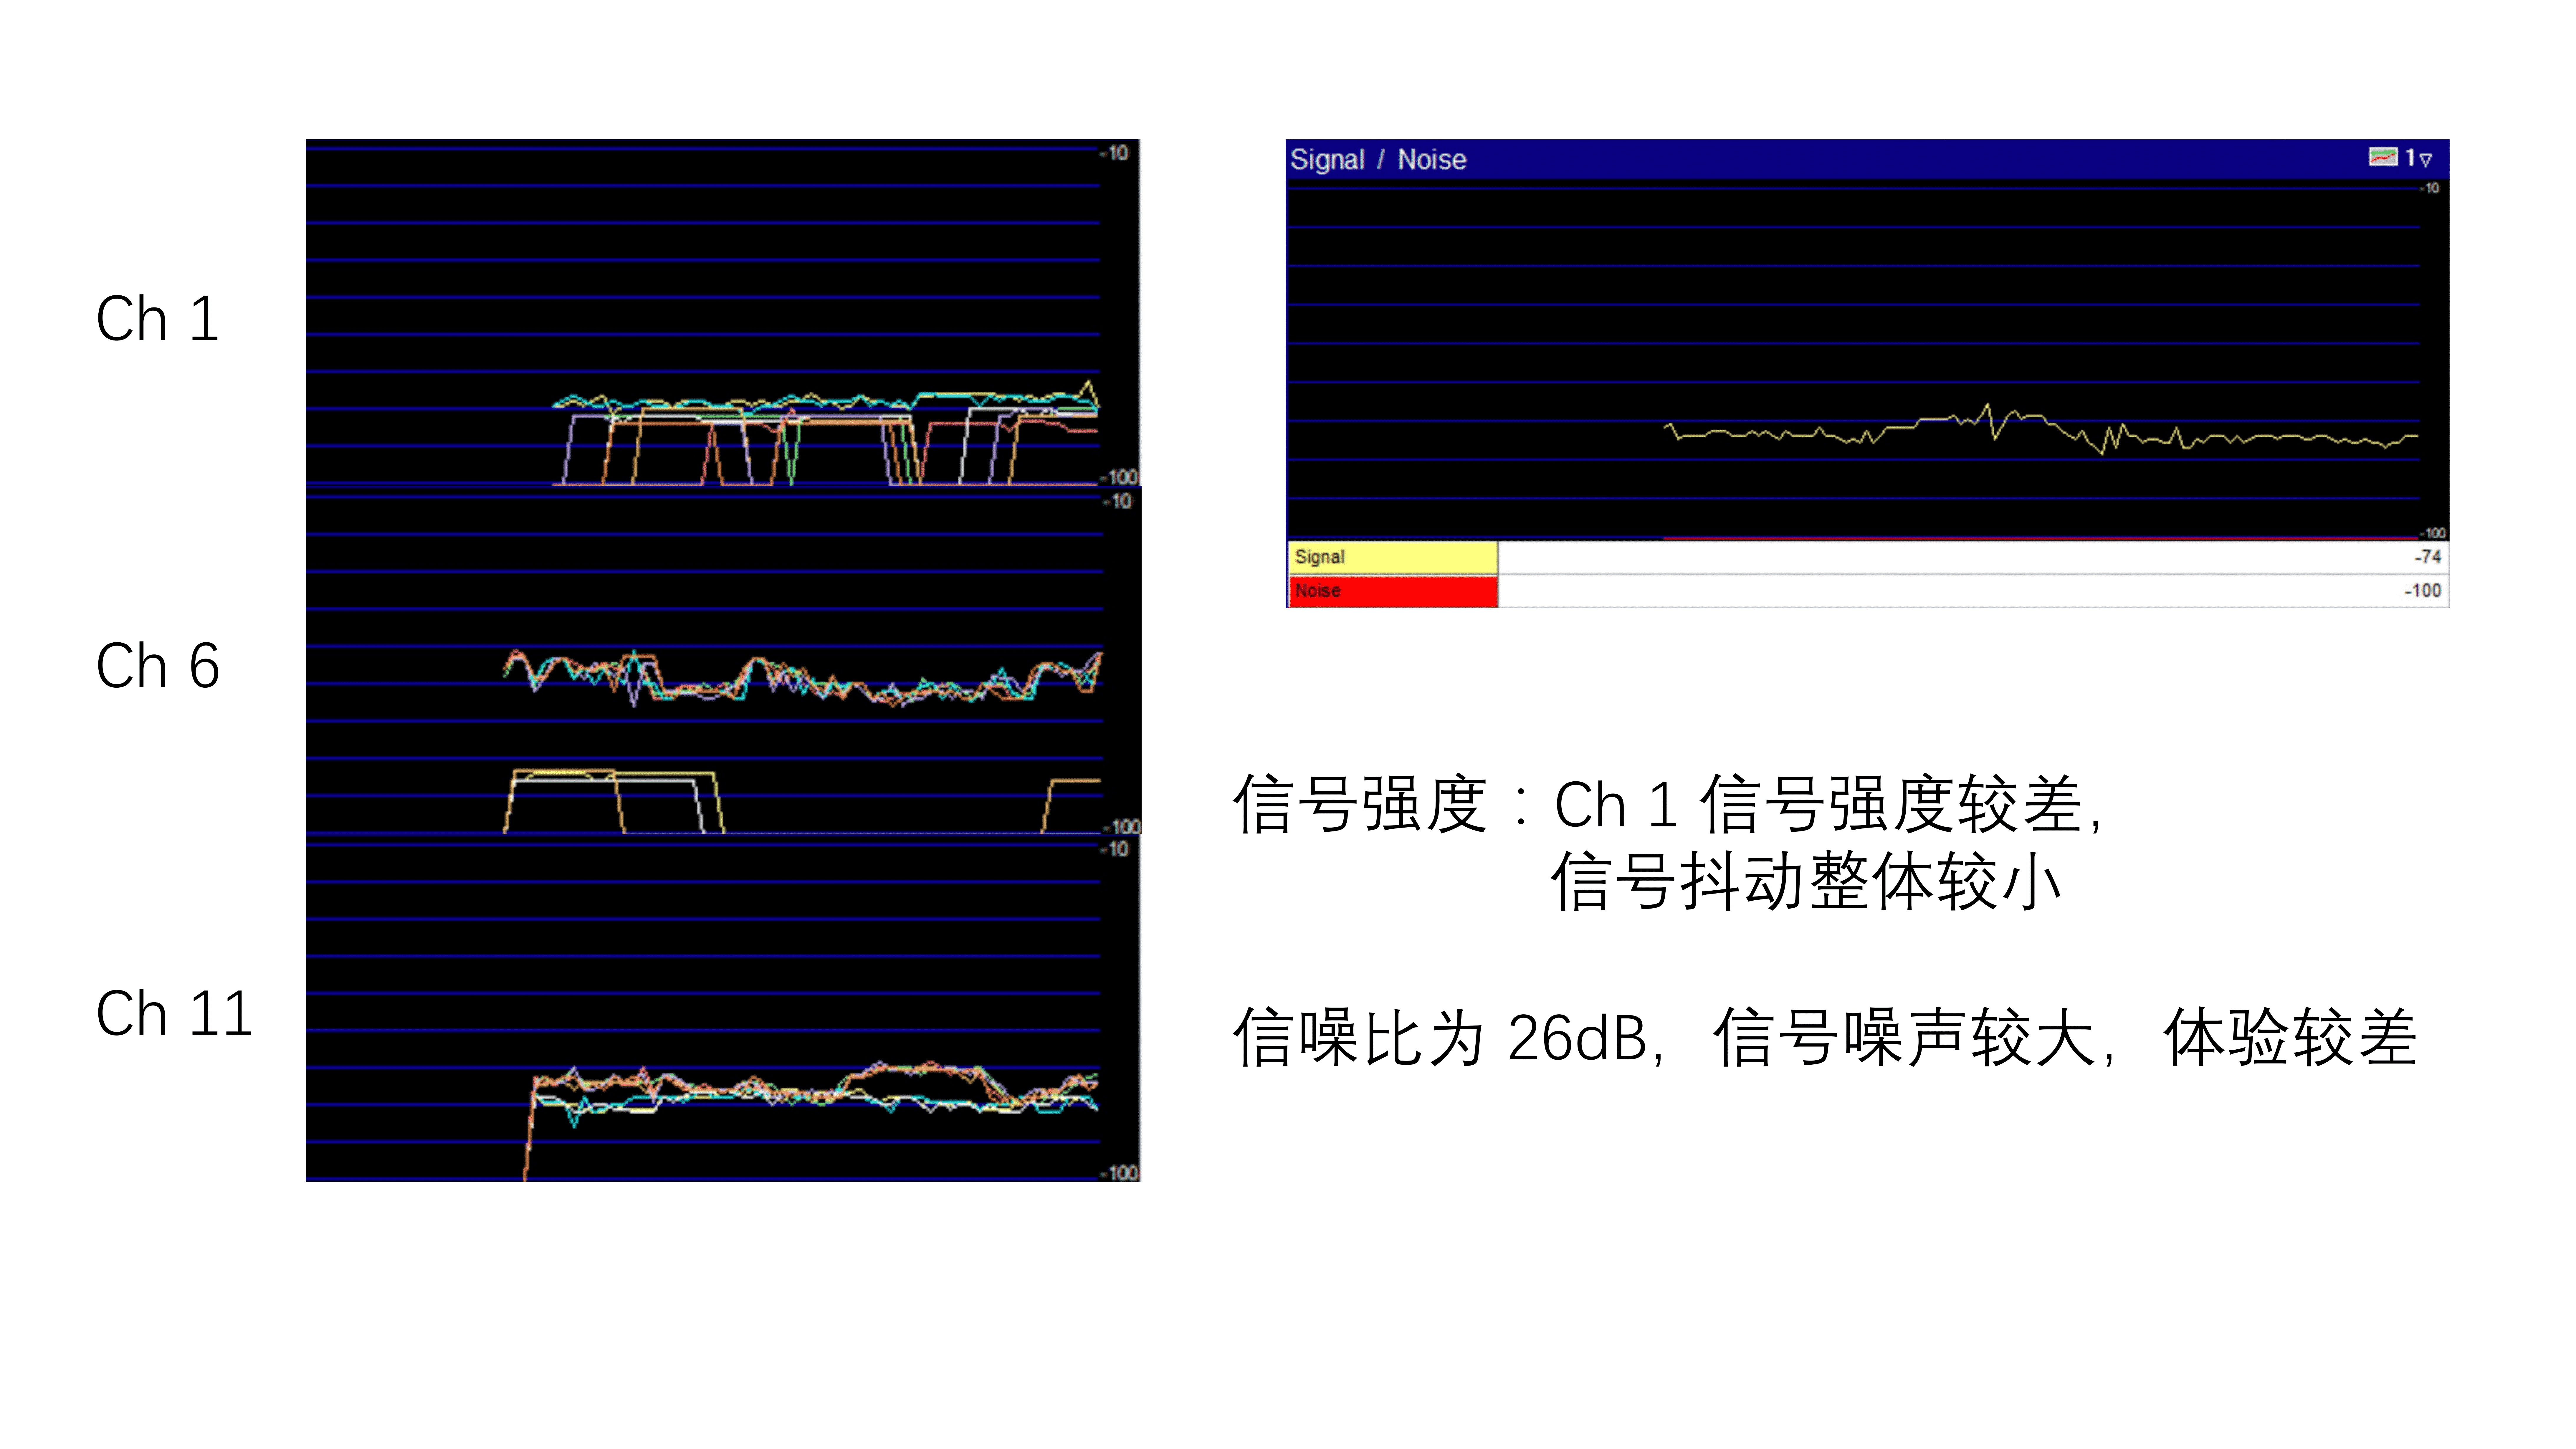
\includegraphics[width=0.9\textwidth]{resources/东北角厕所.png}
    \end{frame}


    \begin{frame}{信道分布状况}
      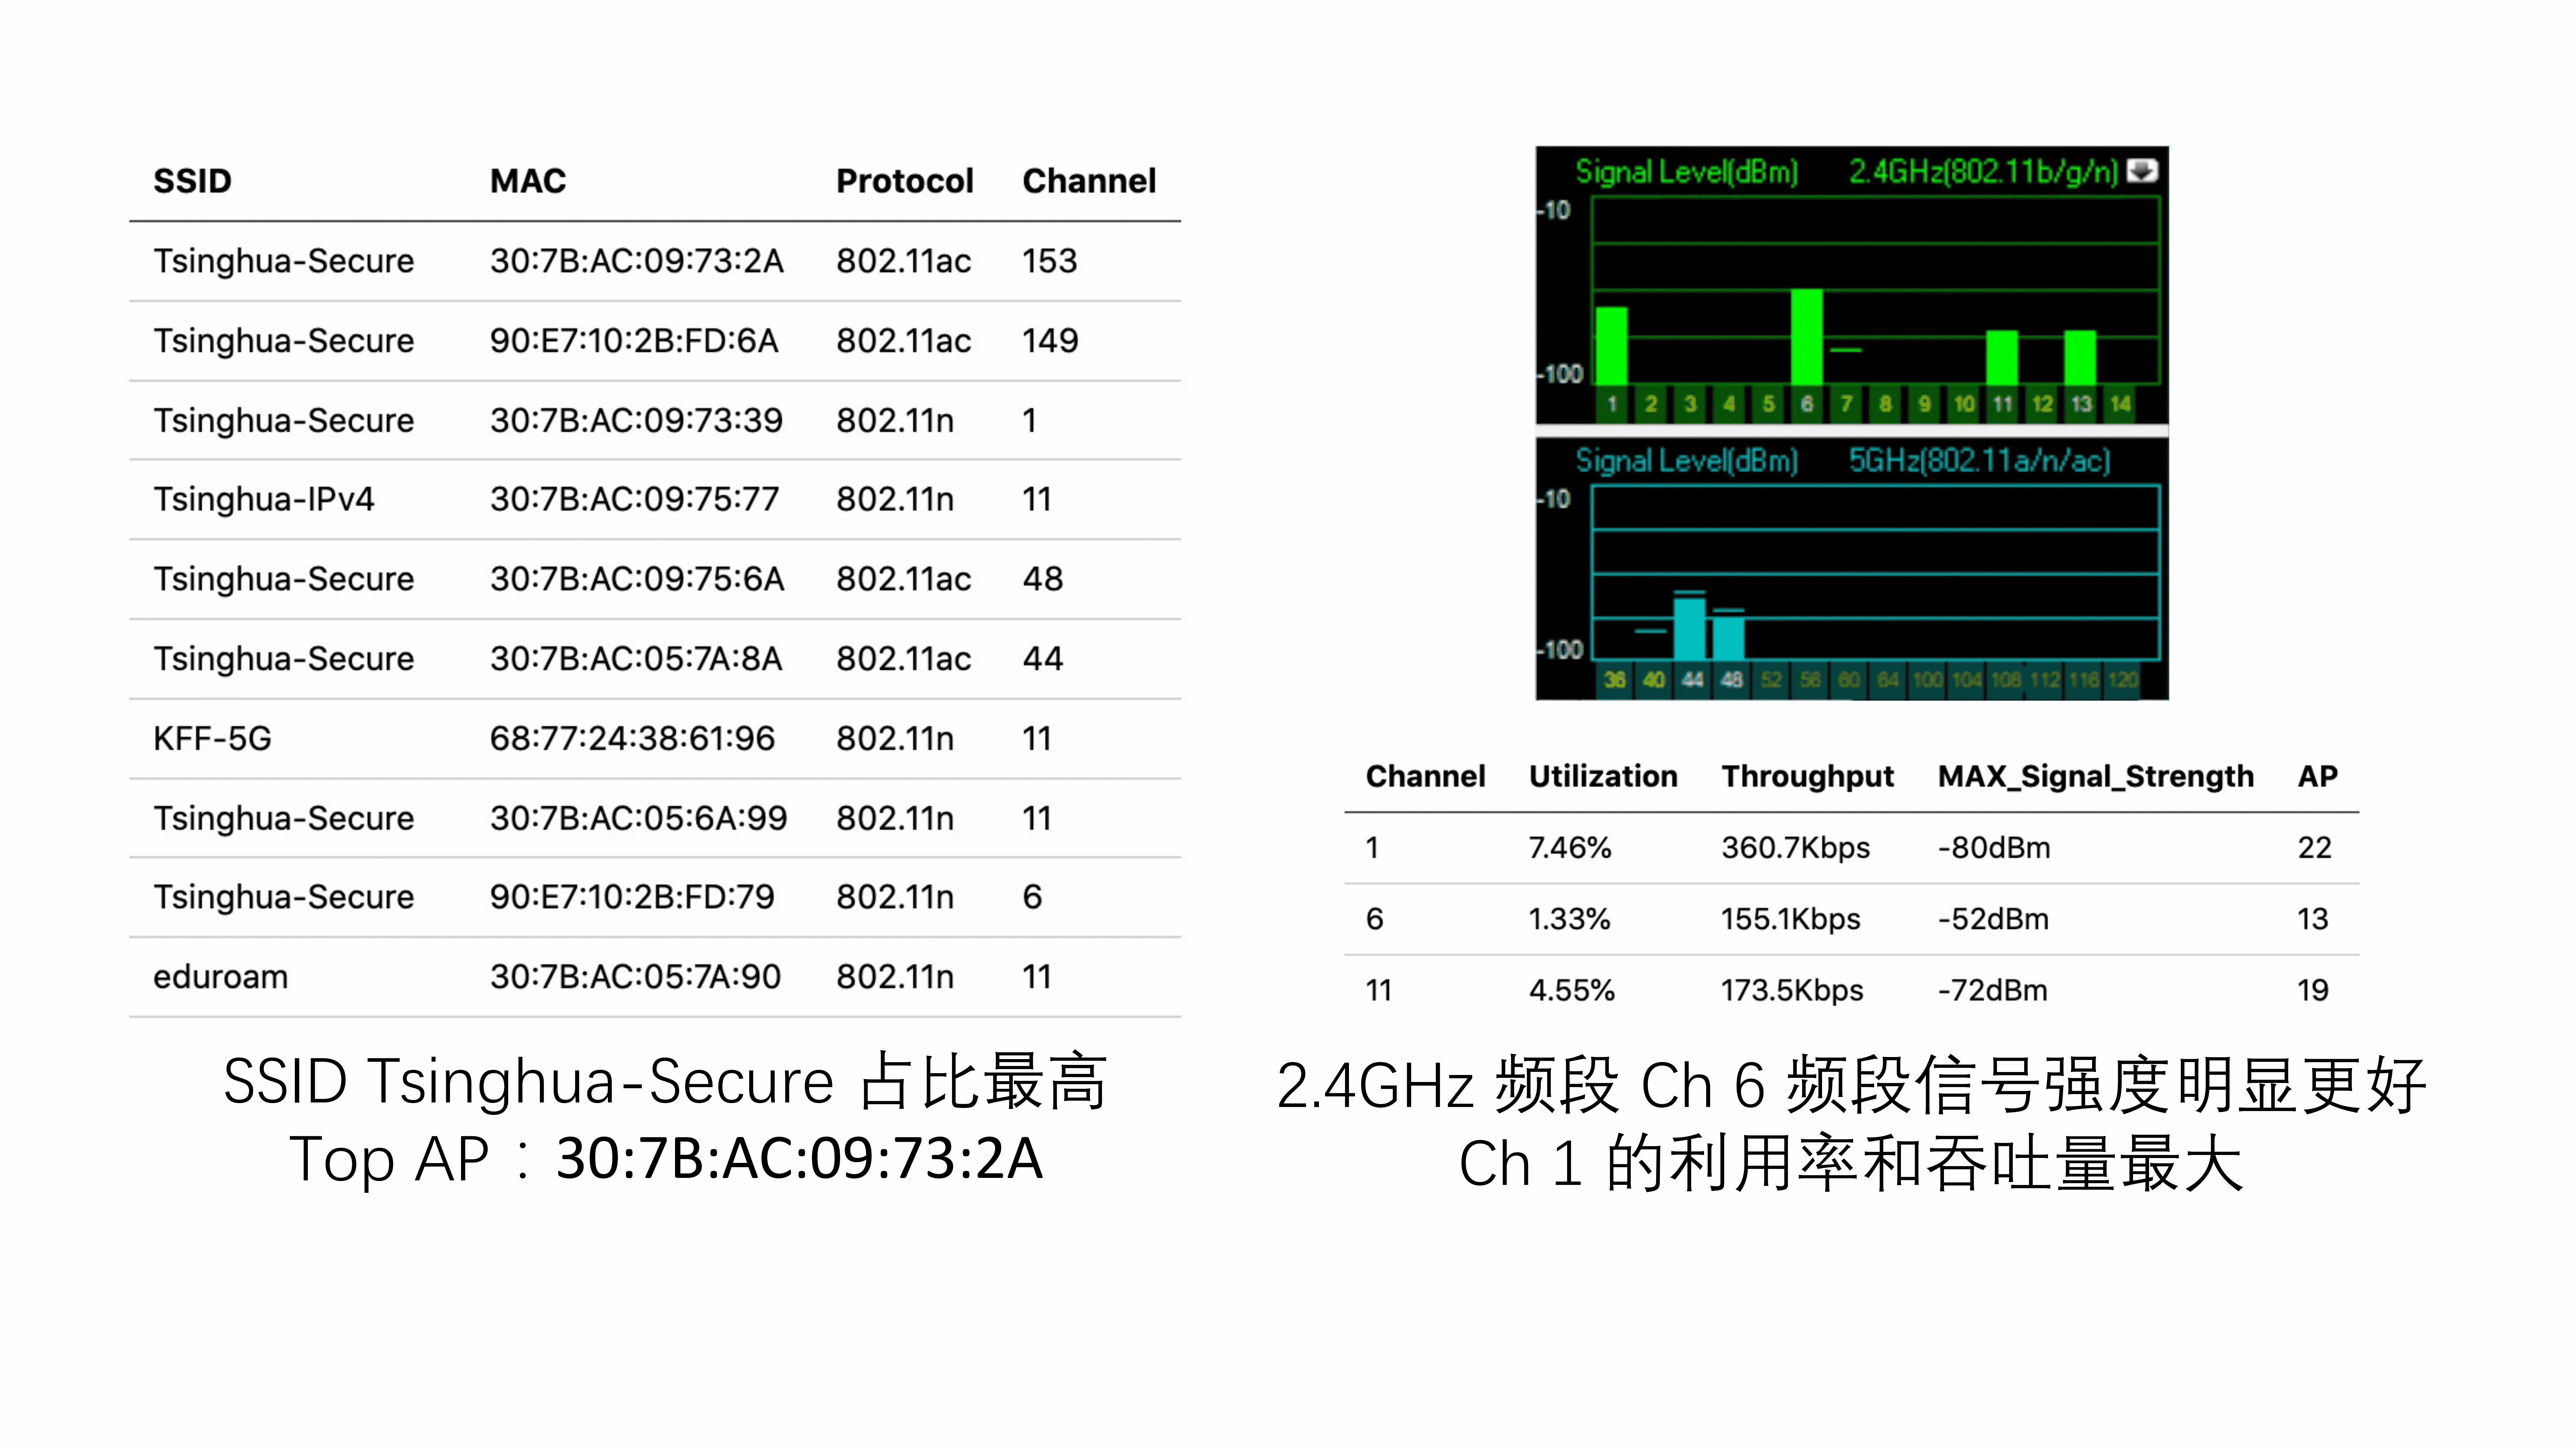
\includegraphics[width=0.9\textwidth]{resources/信道分布情况.png}
    \end{frame}

    \begin{frame}{Top AP: 30:7B:AC:09:73:2A}
      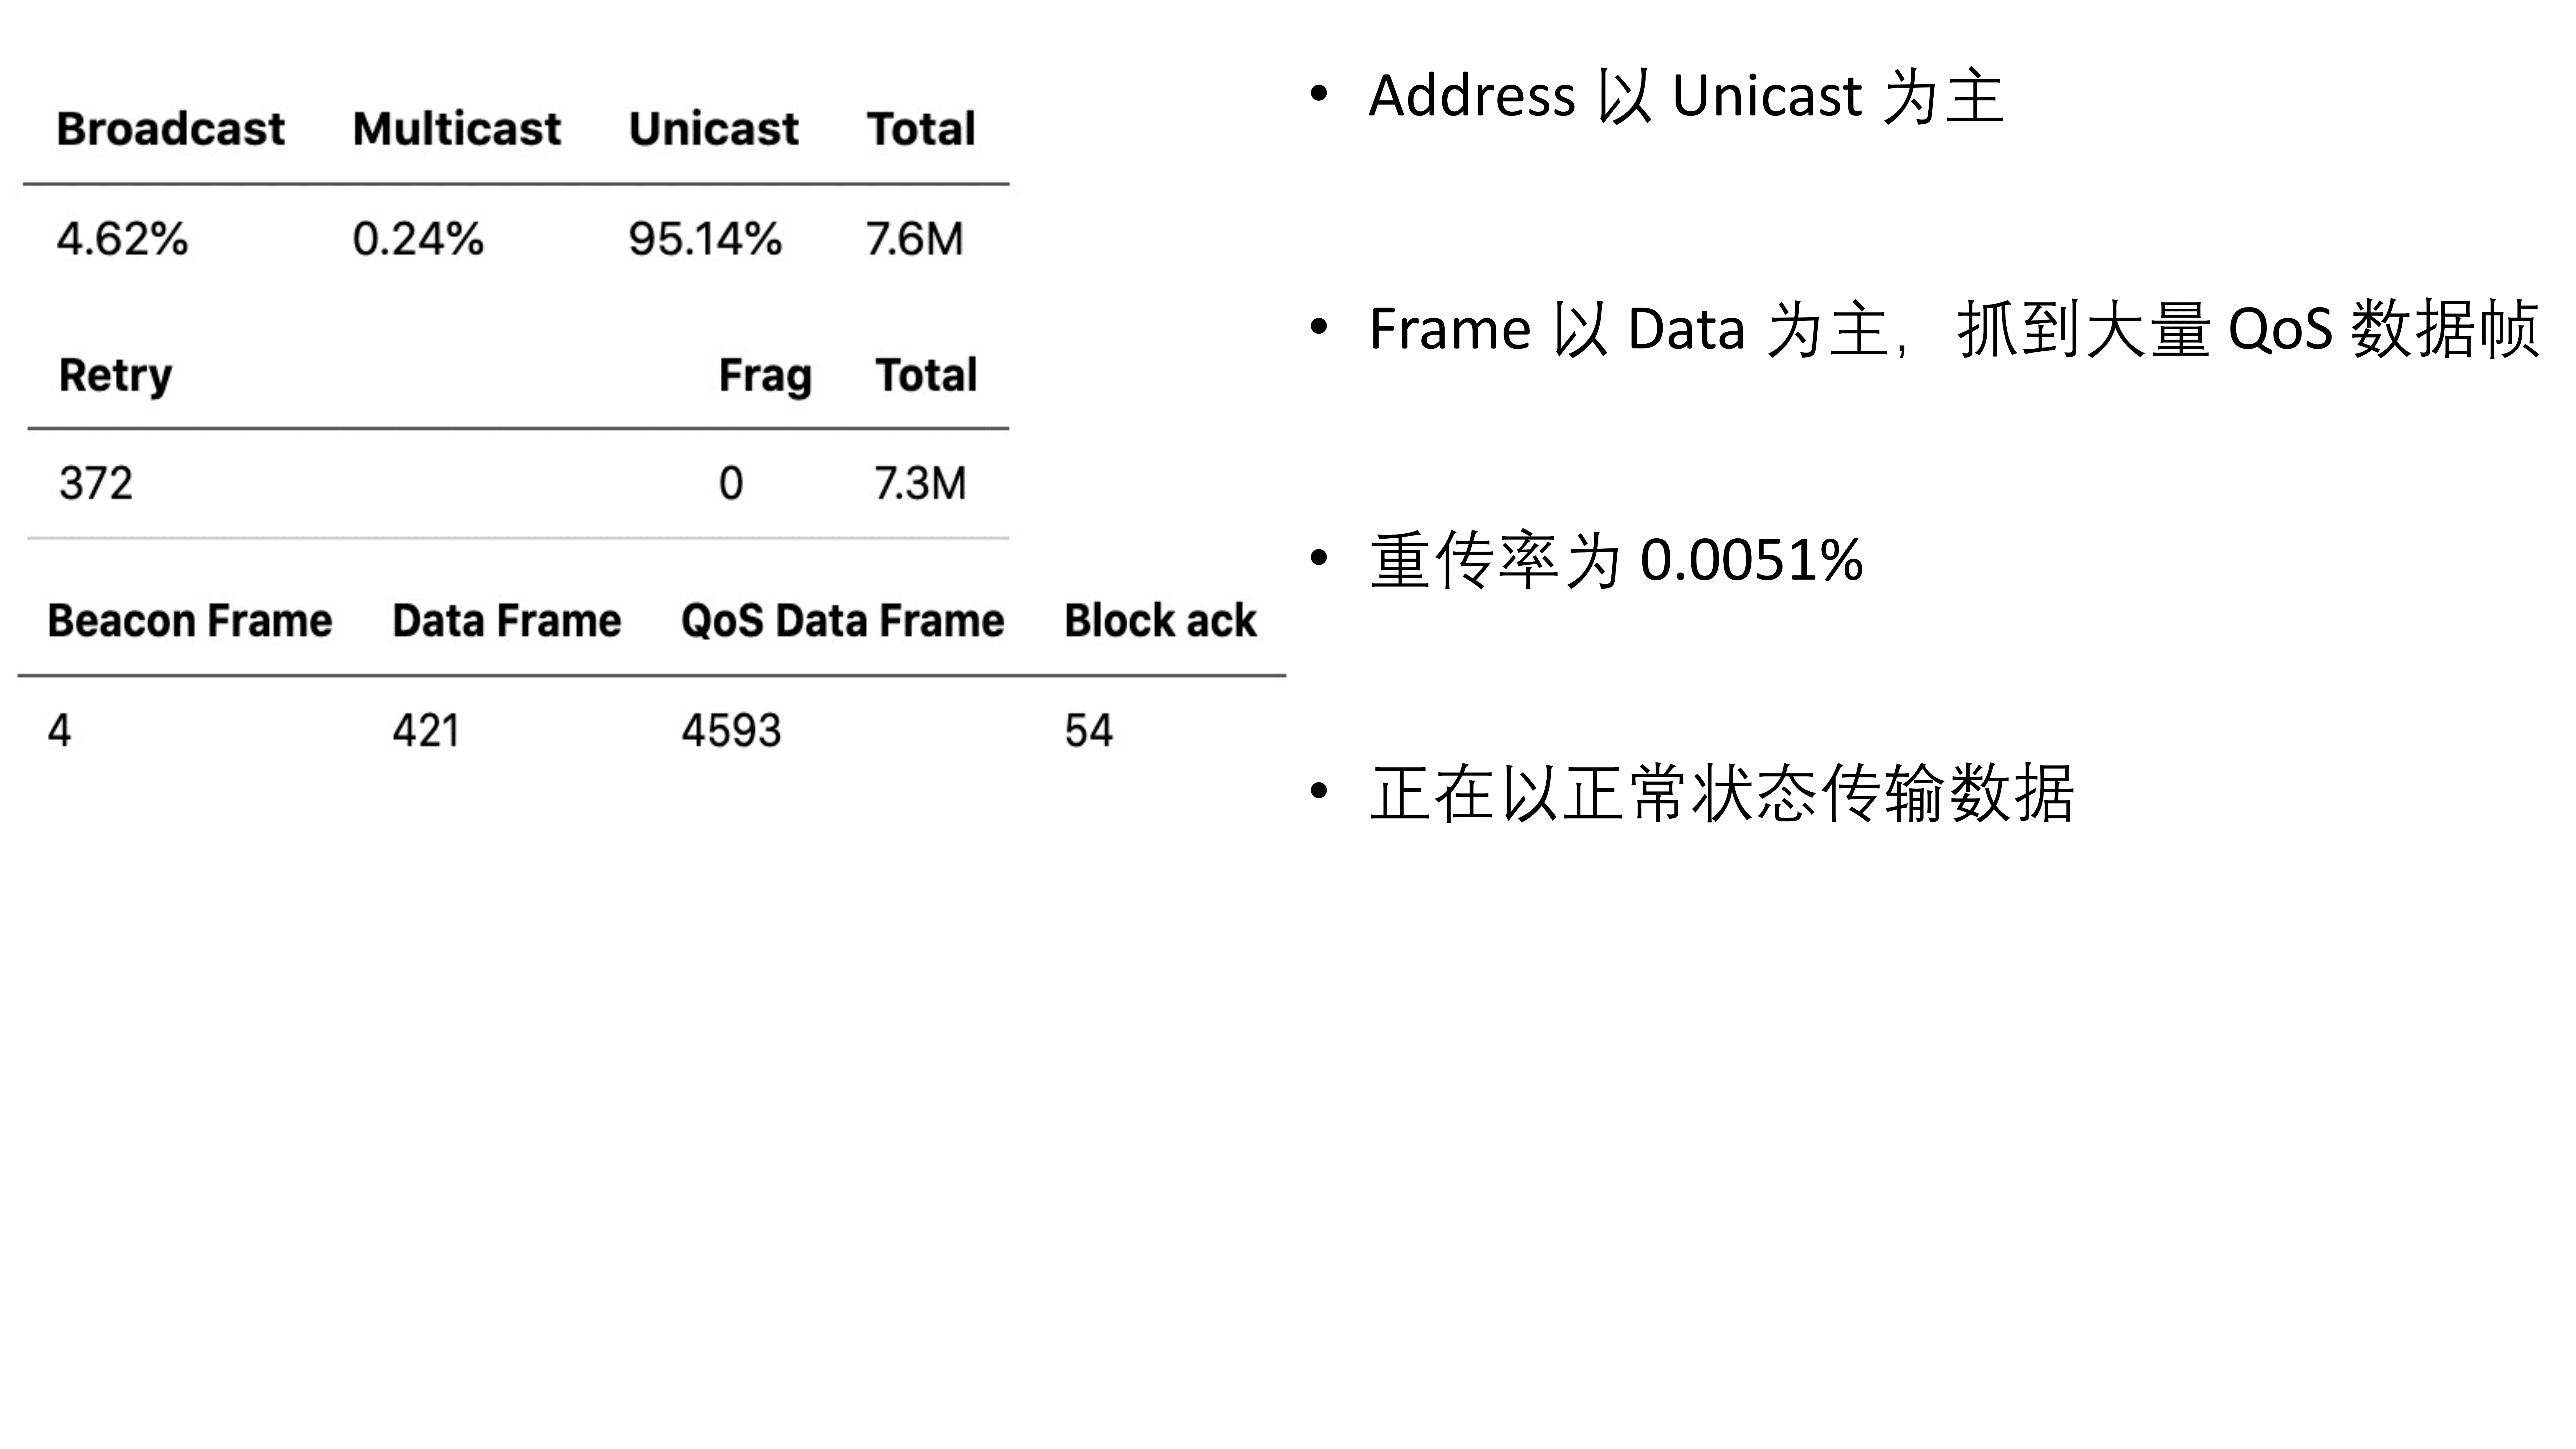
\includegraphics[width=0.9\textwidth]{resources/top AP.png}
    \end{frame}

    \section{字段解析}
    \begin{frame}{典型控制帧}
      \begin{columns}[onlytextwidth]
      \column{.7\textwidth}
      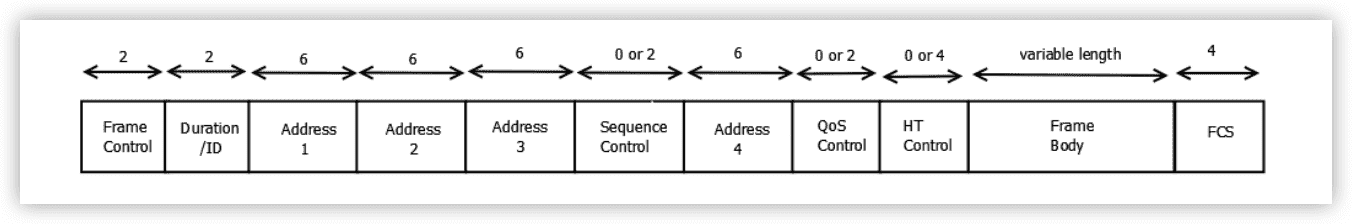
\includegraphics[width=0.8\textwidth]{resources/典型控制帧 1.png}
      \end{columns}
      \begin{columns}[onlytextwidth]
        \column{.5\textwidth}
          \begin{itemize}
           \item Protocol Version:总是 0;
           \item Type / Subtype:Type 定义了该帧是何种类型的帧(数据、控制、管理、扩展);
           \item ToDS / FromDS:指⽰帧的⽬的地是否为传输系统;
           \item More Fragments:指⽰之后是否还有分段;
          \end{itemize}
        \column{.5\textwidth}
          \begin{itemize}
            \item Retry:指⽰是否是重传帧;
            \item Power Mgmt:指定传送端在完成⽬前的基本帧交换之后是否进⼈省电模式;
            \item More Data:设定此位,则代表⾄少有⼀个帧待传送给休眠的⼯作站;
            \item Protected Frame:指⽰帧是否受到链路层安全协议的保护。
          \end{itemize}
      \end{columns}
      \justifying
  \end{frame}

    \begin{frame}{Beacon 帧}
        \begin{columns}[onlytextwidth]
          \column{.6\textwidth}
          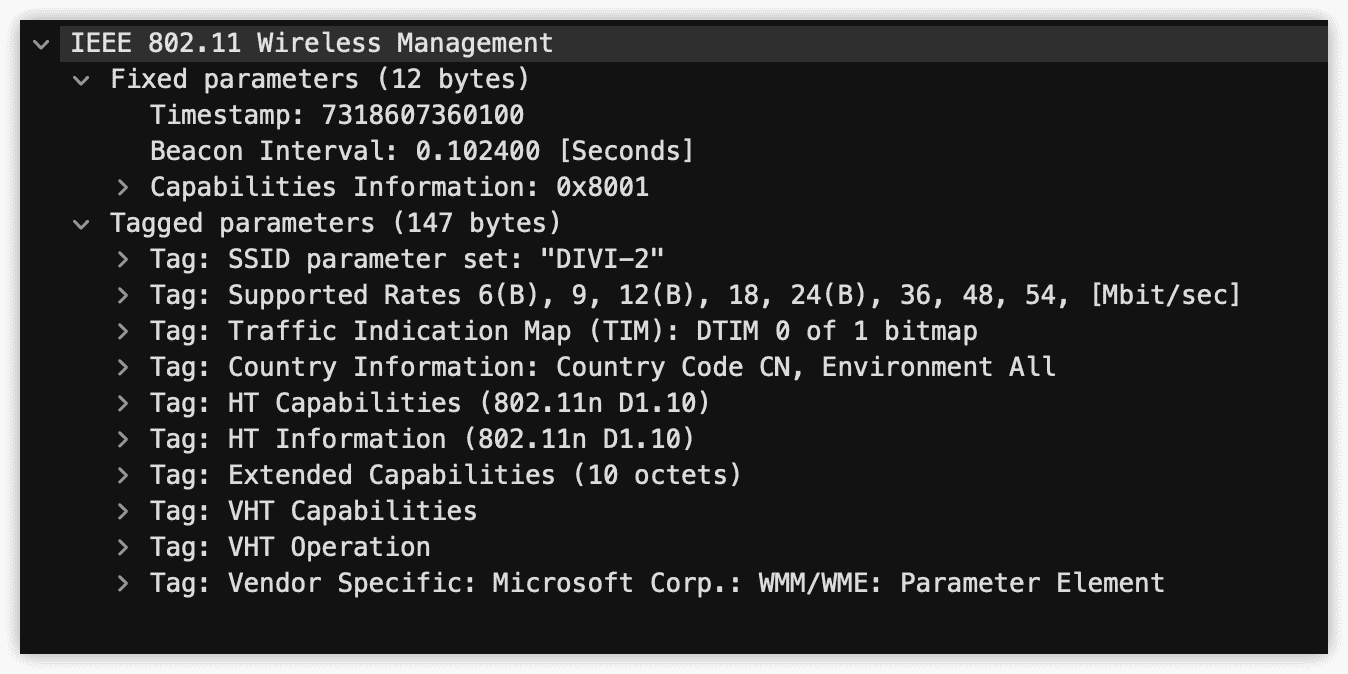
\includegraphics[width=0.8\textwidth]{resources/Beacon.png}
            \begin{itemize}
             \item Timestamp:该 AP 开机以来已经⼯作的时间;
             \item Beacon Interval: 发送⼴播帧的间隔;
             \item Capability Info:⽤来标识⾃⼰是否具有某种功能:每个 bit 各⾃代表⼀个旗标,对应到⽹络所具备的某种特殊功能。⼯作站会使⽤这些数据来判断是否⽀持该 BSS 所有的功能;
            \end{itemize}
          \column{.4\textwidth}
            \begin{itemize}
              \item 如果该字段为 0,则为⼀个 probe request 帧,通过该帧做主动扫描;
              \item Supported Rates:声明所⽀持的速率;
              \item Country Info:国家代号;
              \item VHT Capabilities / VHT Operation:甚⾼吞吐量功能与操作。
            \end{itemize}
        \end{columns}
        \justifying
    \end{frame}

    \begin{frame}{Data 帧与 RTS 帧}
      \begin{columns}[onlytextwidth]
        \column{.5\textwidth}
        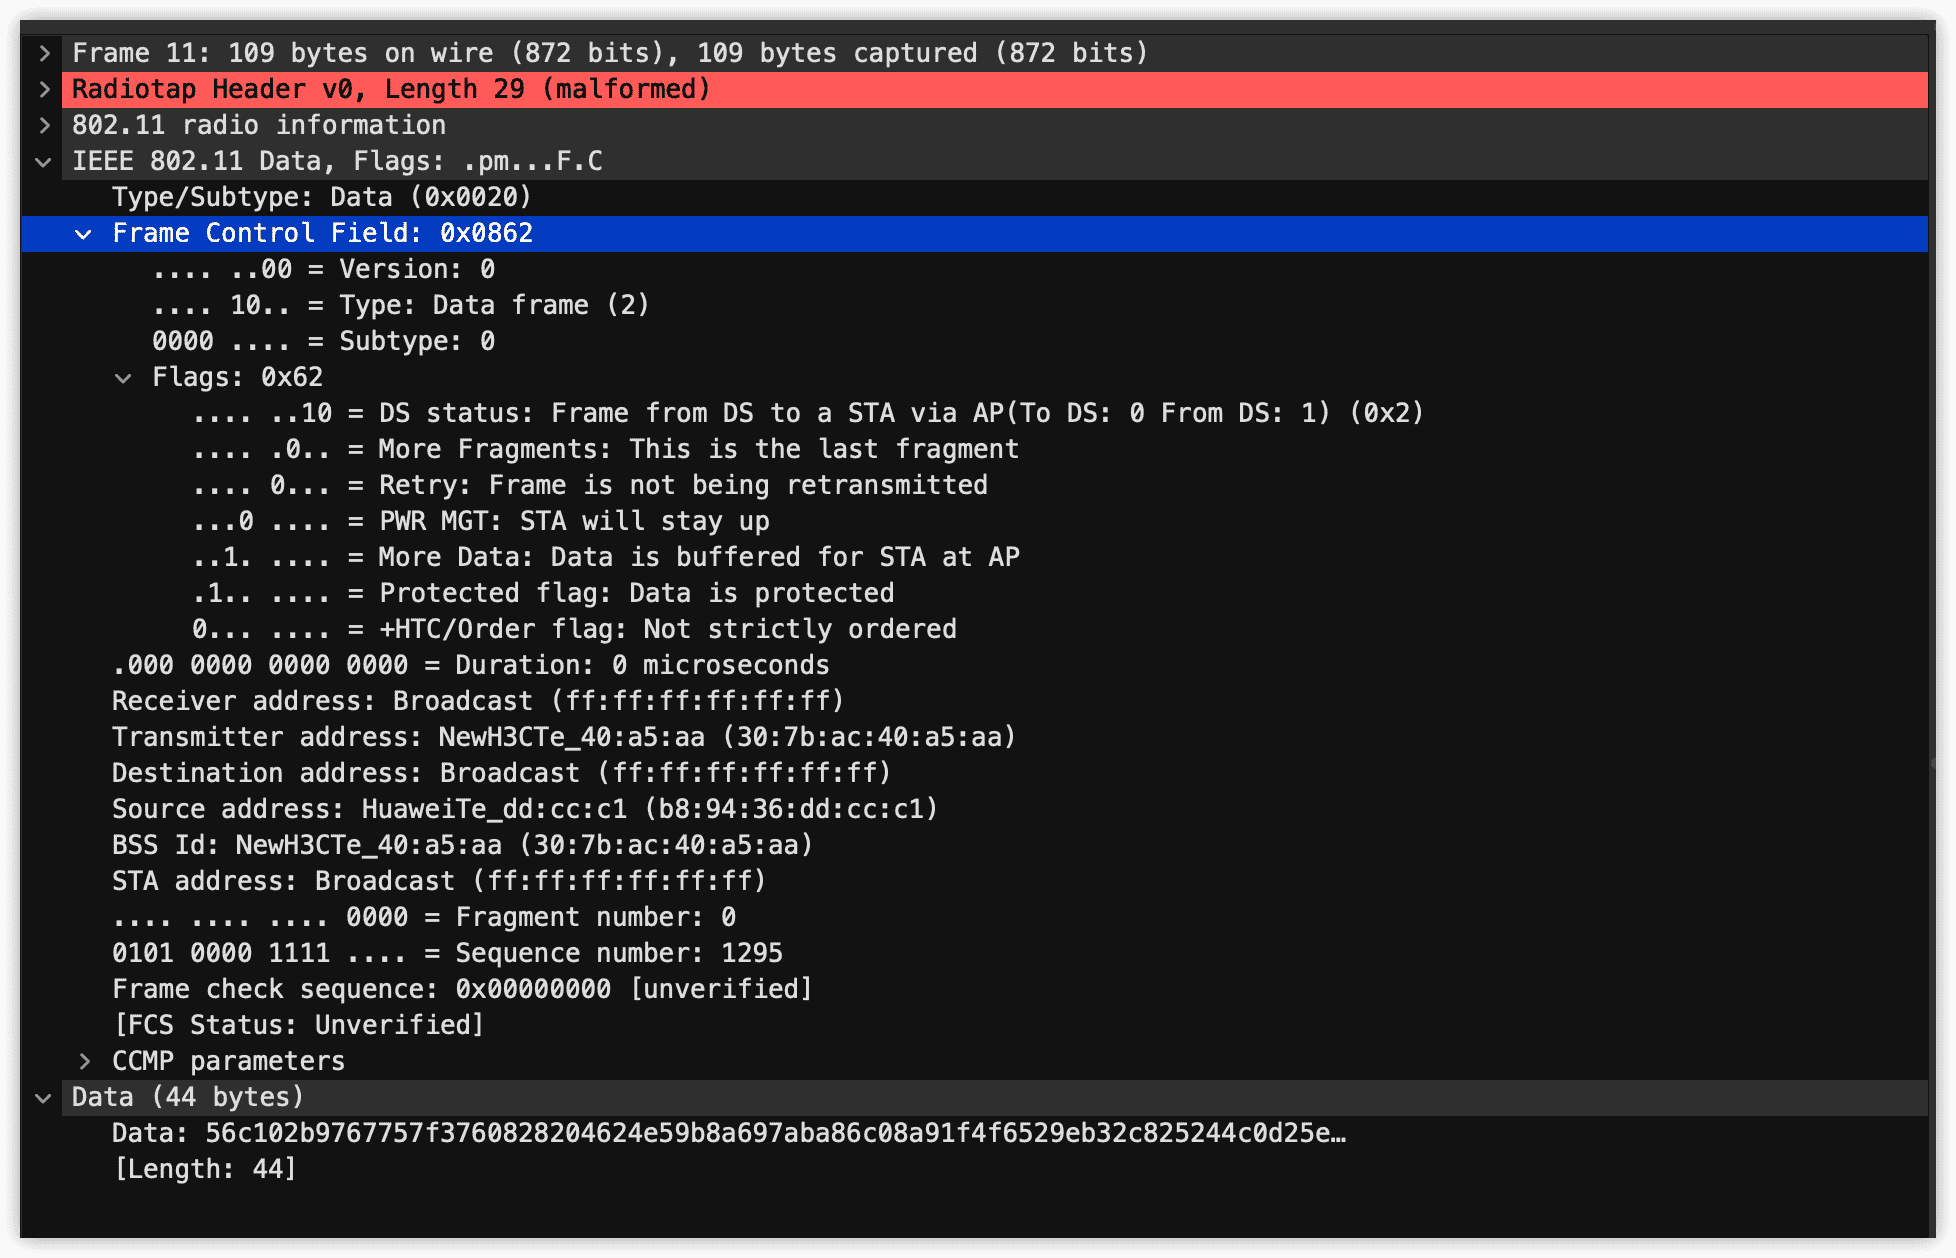
\includegraphics[width=0.8\textwidth]{resources/data.png}
        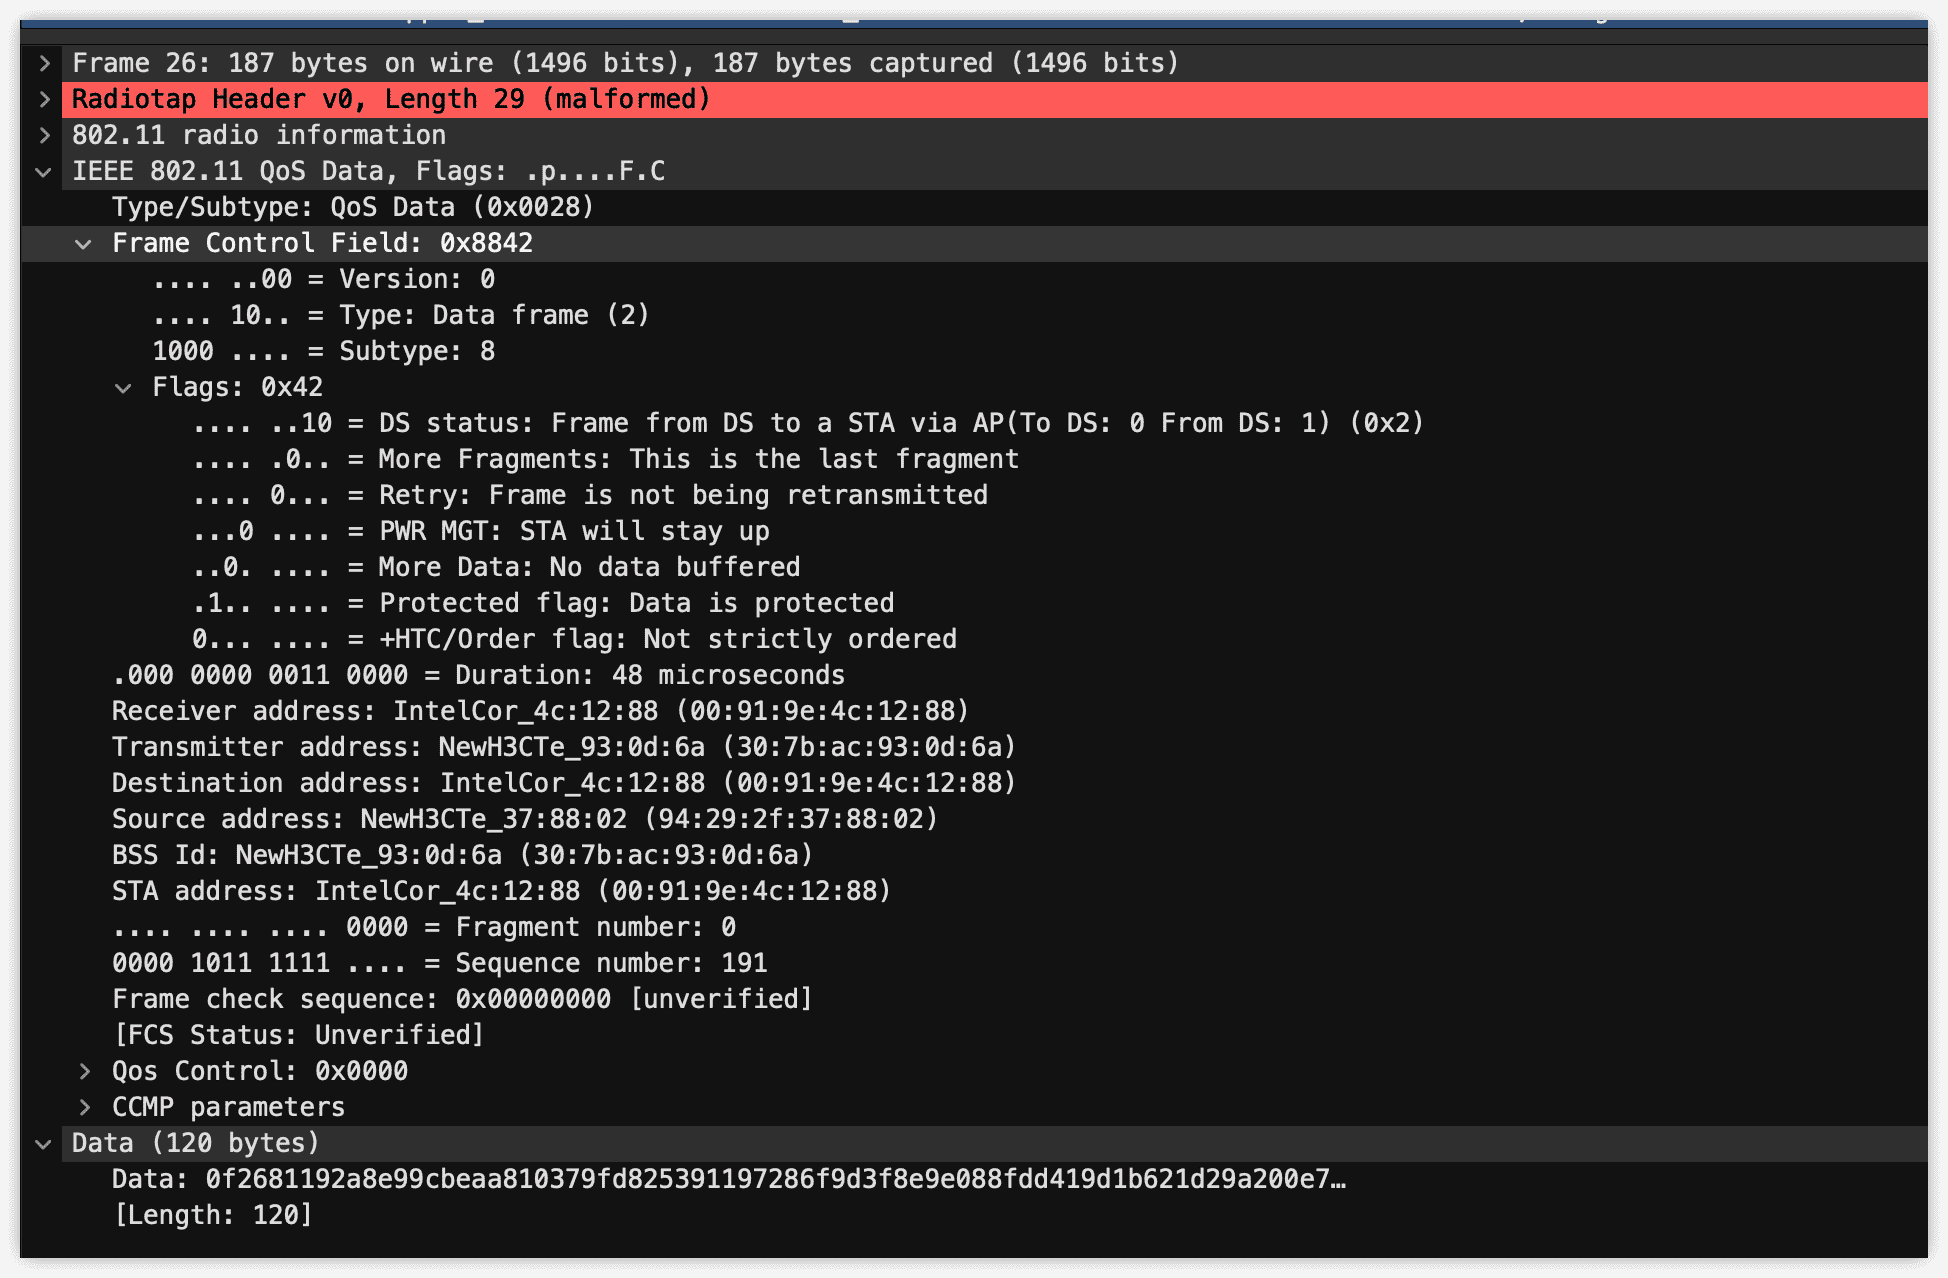
\includegraphics[width=0.8\textwidth]{resources/rts.png}
        \column{.5\textwidth}
          \begin{itemize}
            \item Receiver Address:接收⽅ Mac 地址,这⾥是 AP;
            \item Transmitter Address:发送⽅ Mac 地址,这⾥是⽤户设备;
            \item QoS Control:QoS 的控制字段,某三位指⽰了服务优先级,越低越⾼,这⾥是 0,为最⾼优先级(Best Effort);
            \item Transmitter Address 和 Receiver Address 分别表⽰了 RTS 帧收发⽅的 Mac 地址。
          \end{itemize}
      \end{columns}
      \justifying
    \end{frame}

    \section{统计分析}
    \begin{frame}{统计分析}
      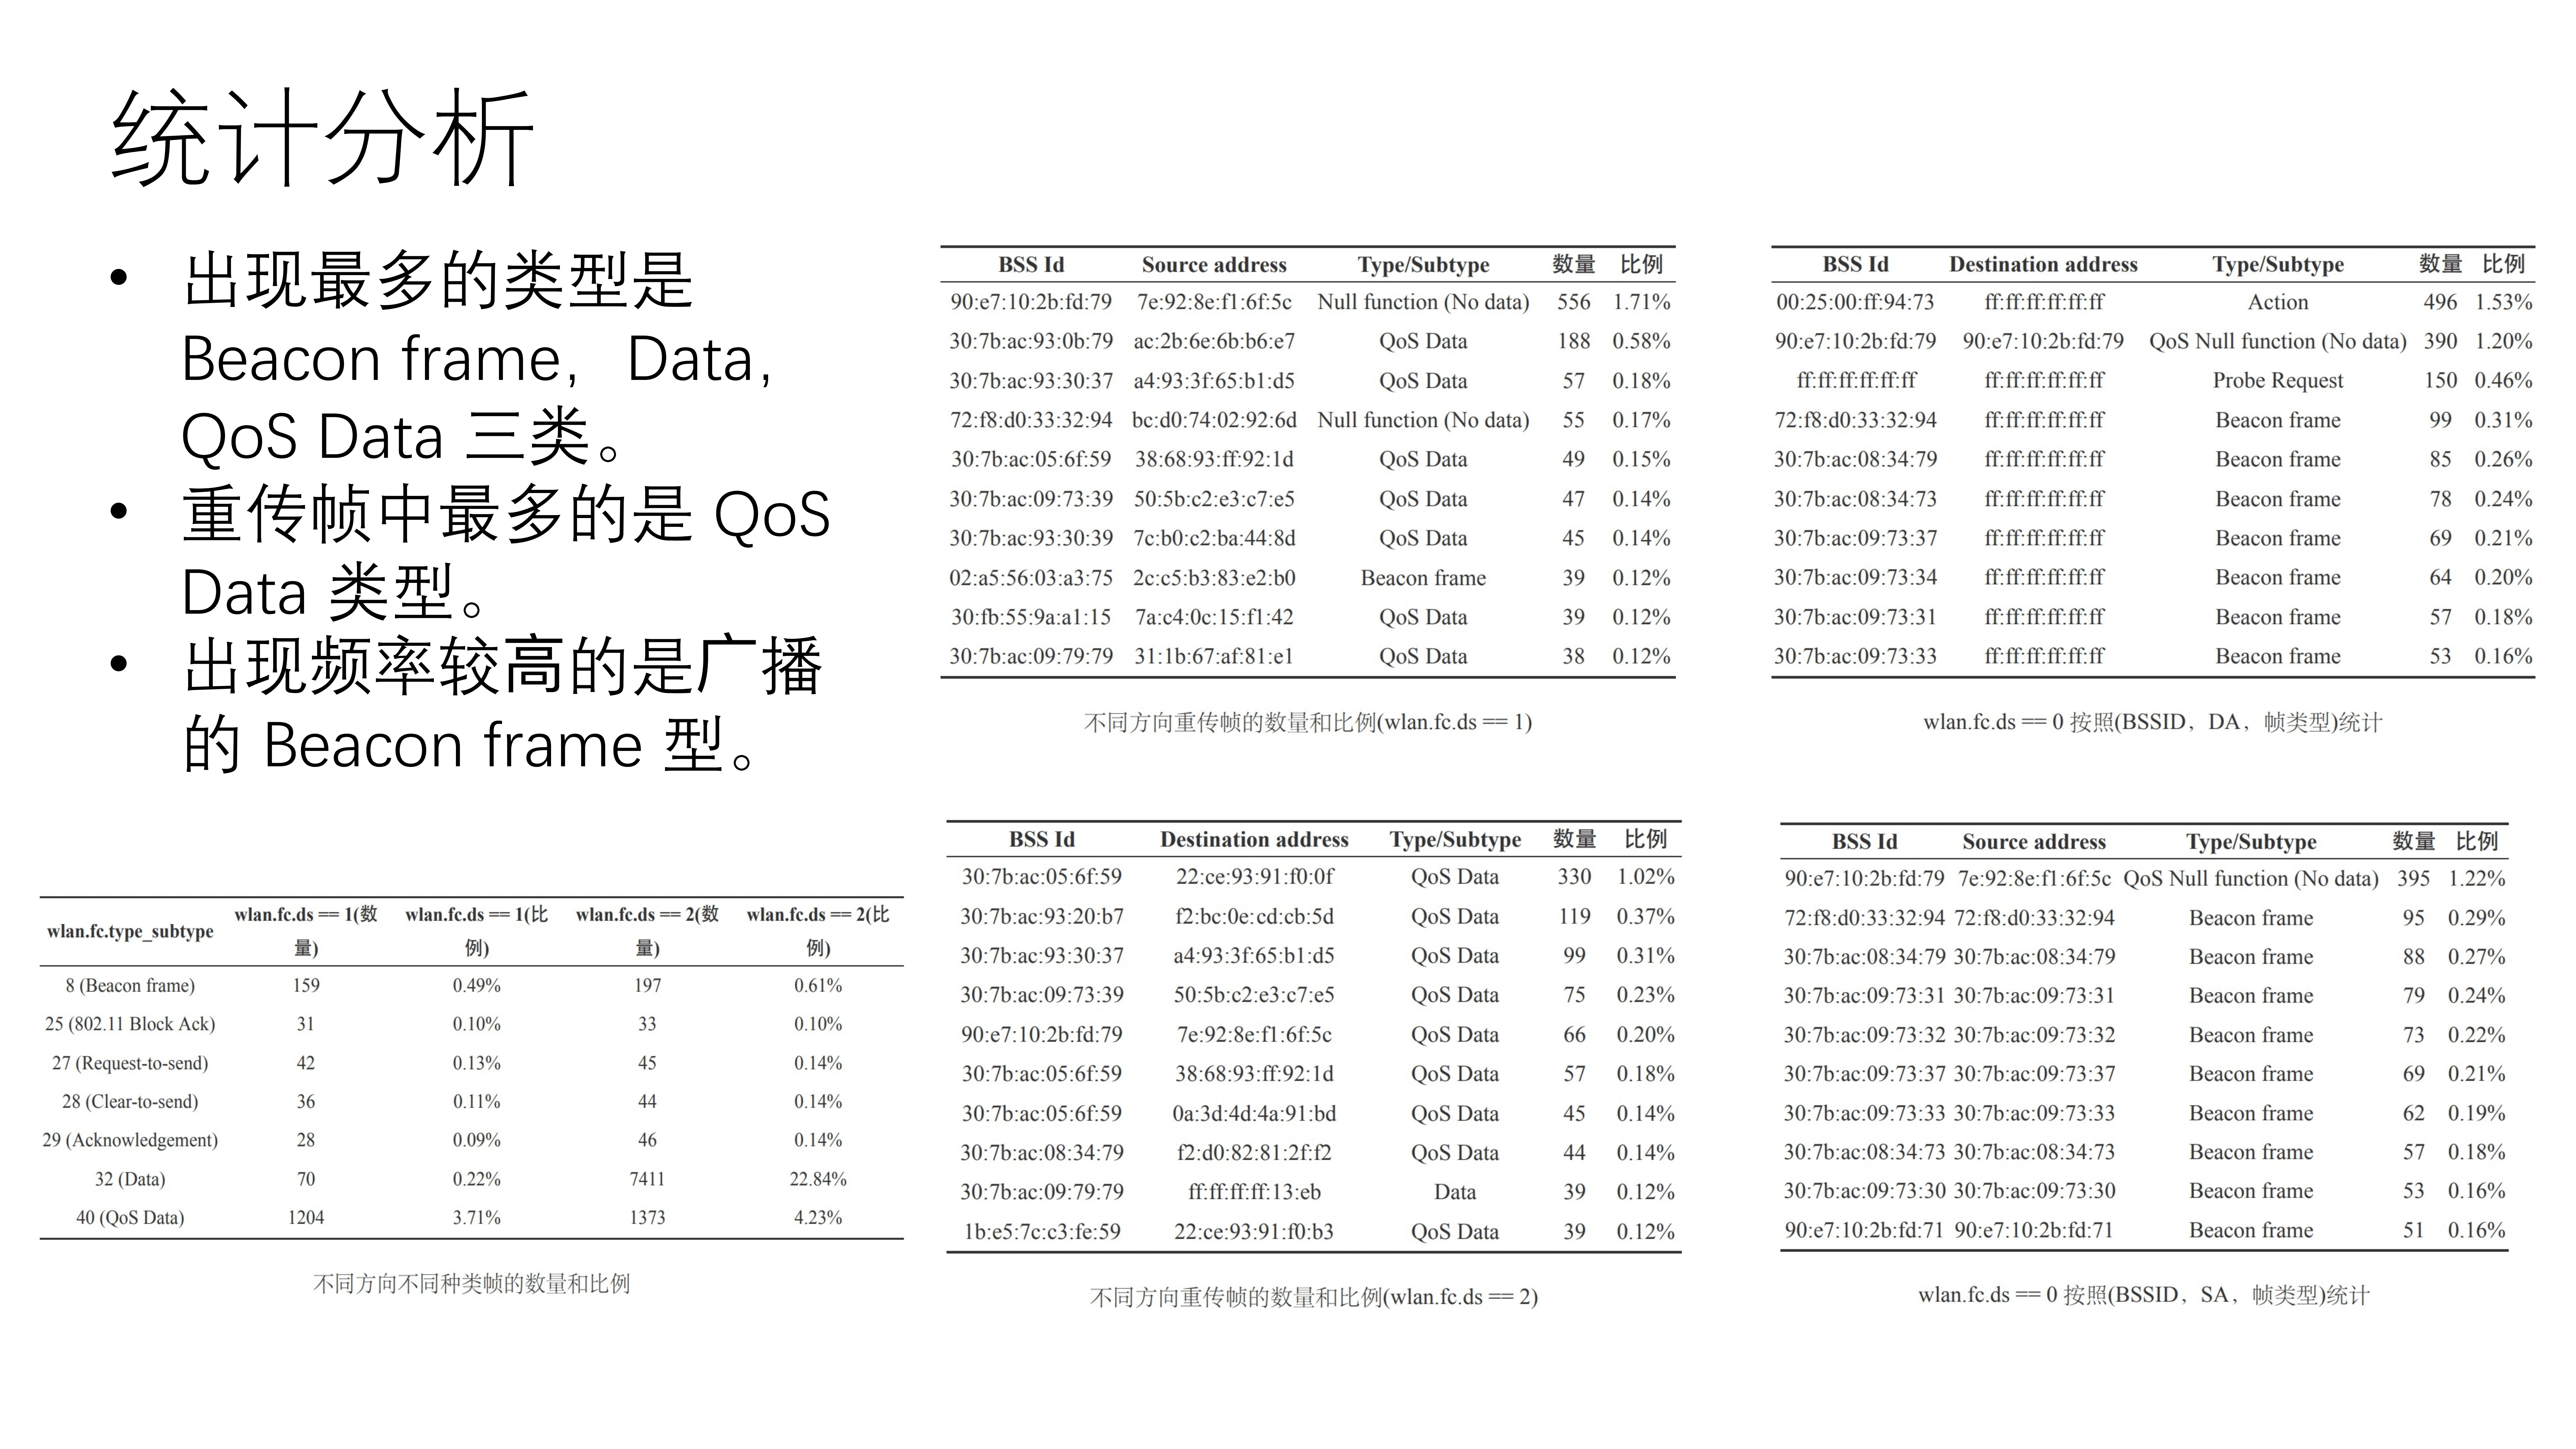
\includegraphics[width=0.9\textwidth]{resources/统计分析.png}
    \end{frame}

    \section{总结感想}
    \begin{frame}{分工总结}
      \begin{columns}[onlytextwidth]
        \column{.5\textwidth}
        测量与统筹:
        \begin{itemize}
          \item 楼层网络勘察——赵晨阳,章管淮,苗恒硕,钏茗喜
          \item Analyzer 监听——苗恒硕,钏茗喜
          \item 时延、吞吐量测试——赵晨阳,章管淮
          \item 统筹工作、调度设备——赵晨阳
          \item 编排报告与汇报文件——赵晨阳
        \end{itemize}
        \column{.5\textwidth}
        报告与分析:
          \begin{itemize}
            \item Analyser 分析网络状况——杜⼦煜
            \item 单 AP 统计分析——杜⼦煜
            \item 802.11 报文解析——赵晨阳
            \item 定点网络分析与监测——章管淮
            \item 信号干扰强度分布——钏茗喜
            \item 楼层总体信号覆盖、具体信号强度分析——苗恒硕,钏茗喜
            \item 抓包统计分析——苗恒硕,赵晨阳
          \end{itemize}
      \end{columns}
    \end{frame}

    \begin{frame}{困难感悟}
      \begin{columns}[onlytextwidth]
        \column{.5\textwidth}
        困难:
        \begin{itemize}
          \item 由于疫情影响,我们全组同学感染,报告编写遇到了非常大的阻碍。
          \item 此外,小组成员对于 Analyser 此类工业系统软件操作不够熟悉,也难以线下交流解决方案。
          \item 最终,我们两次借用实验设备,在助教与老师耐心负责的指导和解答圆满完成了报告,交上了满意的答卷!
        \end{itemize}
        \column{.5\textwidth}
        感悟:
          \begin{itemize}
            \item 小组成员初次使用 Analyzer 和 Surveyor 对课程所学习的无线移动网络技术进行了实地分析。
            \item 实际体会到了图书馆环境下的无线网络工作情况,加深了对于网络原理知识的理解,掌握了勘察并分析优化无线网络的许多方法。
            \item 希望今后我们也能将更多技术应用于实际,让科技带来变革和价值。
          \end{itemize}
      \end{columns}
    \end{frame}
\end{document}
